\subsection{Planes and Surfaces}
\subsubsection{Plane in $\mathbb{R}^3$}
Given a fixed point $P_0$ and a nonzero \textbf{normal vector n}, the set of points $P$ in $\mathbb{R}^3$ for which $\vec{P_0 P}$ is orthogonal to $\mathbf{n}$ is called a \textbf{plane}.

\subsubsection{General Equation of a Plane in $\mathbb{R}^3$}
The plane passing through the point $P_0 (x_0,\, y_0,\, z_0)$ with a nonzero normal vector $\mathbf{n} = \langle a,\, b,\, c \rangle$ is described by the equation

\begin{equation}
    a(x - x_0) + b(y - y_0) + c(z - z_0) = 0 \quad \text{or} \quad ax + by + cz = d
\end{equation}

where $d = ax_0 + by_0 + cz_0$.

\subsubsection{Parallel and Orthogonal Planes}
Two distinct planes are \textbf{parallel} if their respective normal vectors are parallel (that is, the normal vectors are scalar multiples of each other). Two planes are \textbf{orthogonal} if their respective normal vectors are orthogonal (that is, the dot product of the normal vectors is zero).

\subsubsection{Cylinder}
Given a curve $C$ in a plane $P$ and a line $\ell$ not in $P$, a \textbf{cylinder} is the surface consisting of all lines parallel to $\ell$ that pass through $C$.

\subsubsection{Trace}
A \textbf{trace} of a surface is the set of points at which the surface intersects a plane that is parallel to one of the coordinate planes. The trace in the coordinate planes are called \textbf{xy-trace}, the \textbf{xz-trace}, and the \textbf{yz-trace}.

\subsubsection{Quadratic Surfaces}
\begin{tabularx}{\linewidth}{|c|c|X|}
    \hline
    \textbf{Name} & \textbf{Standard Equation} & \textbf{Features} \\ \hline
    Ellipsoid                   & $\frac{x^2}{a^2} + \frac{y^2}{b^2} + \frac{z^2}{c^2} = 1$     & All traces are ellipses. \\ \hline
    Elliptic paraboloid         & $z = \frac{x^2}{a^2} + \frac{y^2}{b^2}$                       & Traces with $z = z_0 > 0$ are ellipses. Traces with $ x = x_0$ or $y = y_0$ are parabolas. \\ \hline
    Hyperboloid of one sheet    & $\frac{x^2}{a^2} + \frac{y^2}{b^2} - \frac{z^2}{c^2} = 1$     & Traces with $z = z_0$ are ellipses for all $z_0$. Traces with $x = x_0$ or $y = y_0$ are hyperbolas. \\ \hline
    Hyperboloid of two sheets   & $-\frac{x^2}{a^2} - \frac{y^2}{b^2} + \frac{z^2}{c^2} = 1$    & Traces with $z = z_0$ with $|z_0| > |c|$ are ellipses. Traces with $x = x_0$ and $y = y_0$ are hyperbolas. \\ \hline
    Elliptic cone               & $-\frac{x^2}{a^2} + \frac{y^2}{b^2} = \frac{z^2}{c^2}$        & Traces with $z = z_0 \neq 0$ are ellipses. Traces with $x = x_0$ or $y = y_0$ are hyperbolas or intersecting lines. \\ \hline
    Hyperbolic paraboloid       & $z = \frac{x^2}{a^2} - \frac{y^2}{b^2}$                       & Traces with $z = z_0 \neq 0$ are hyperbolas. Traces with $x = x_0$ or $y = y_0$ are parabolas. \\ \hline
\end{tabularx}

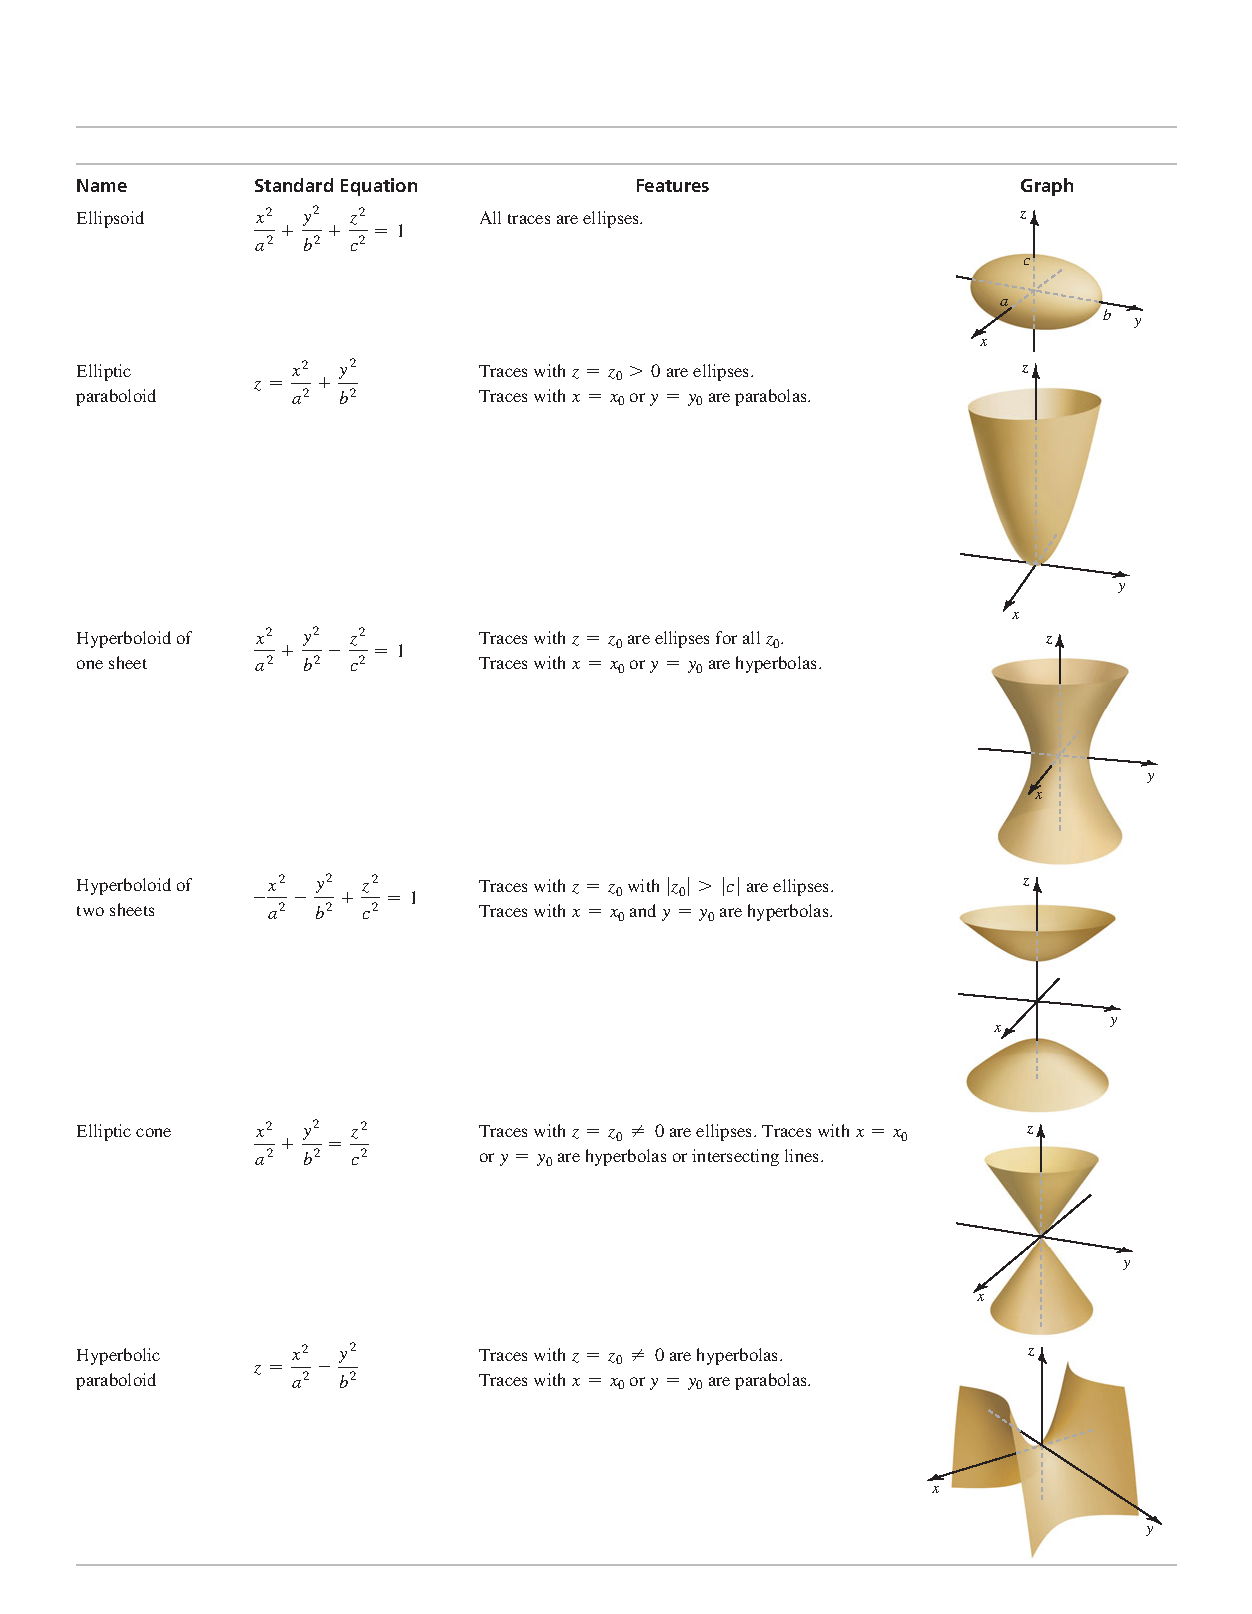
\includepdf{assets/planes-and-surfaces}
